\definecolor{vmcol}{RGB}{150,150,150}
\definecolor{nmcol}{RGB}{200,200,200}
\definecolor{zscol}{RGB}{83,142,213} % red: 217,151,149
\definecolor{zicol}{RGB}{194,214,154}

\newcommand{\zs}[0]{\cellcolor{zscol}}				% soll
\newcommand{\zi}[0]{\cellcolor{zicol}}				% ist
%\newcommand{\ms}[0]{\makebox[.613cm][r]{$\blacklozenge$}}	% Meilenstein
\newcommand{\ms}[1]{
	\makebox[.7cm][r]{
		\tikz[baseline=(char.base)]{
			\node[shape=circle,draw,inner sep=.02cm,fill=black,text=white] (char) { #1 };
		}
	}
}

\newcommand{\sq}[1]{\textcolor{#1}{\rule{.3cm}{.3cm}}}

\newcommand{\phase}[1]{
	\multicolumn{22}{l}{} \\
	\multicolumn{22}{l}{\cellcolor{gray!20}\textbf{#1}} \\ \hline
}

\chapter{Project Plan}
In this chapter we are going to describe several aspects regarding the planing of our project, such as our project methods, the requirements and use cases as well as a short concept of our application. 
\section{Project Method}
Since this wasn't a project where the project scope and goals were strictly defined and clear from the beginning, it was very important to elaborate the requirements in close collaboration with our supervisors early on. This is why we decided our project would be very suitable for an agile kind of project method. Because of the small team, consisting of only two members, we didn't chose a particular project method like SCRUM, as this would have probably caused more overhead than actual benefits.  

We have therefore set up regular meetings (usually once every 2 weeks) with our supervisors to discuss our ideas and get feedback about the current progress.

\section{Requirements}
As the first step, we have elaborated the goals and requirements for our application. We have structured the requirements into groups that correspond to the actors of the CHVote protocol and therefore the views our application is going to consist of.

Some requirements affect multiple or all actors and are therefore listed as "`General Requirements"'. We have also added a priority and requirement type to simplify the planing and time management.
\subsection{General Requirements}
\begin{longtable}{p{0.5cm}p{9cm}p{1cm}p{1cm}p{1cm}p{1cm}}
\hline
 & Description & Type & Prio. & Phase & Status\\
\hline
R1 & The CHVote protocol is implemented as specified in the latest specification document. The only exclusion are the algorithms for channel security. & Must & High & 1 & Done\\
R2 & The application is web-based shows updates within the same demo-election in real-time. & Must & High & 1 & Done\\
R3 & The system supports 1-out-of-3 type of elections (e.g. elect 1 of 3 possible candidates) & Must & High & 1 & Done\\
R4 & The system supports multiple parallel elections & Must & High & 1 & \\
R5 & Users can create new elections & Must & High & 1 & Done \\
R6 & The system supports internationalization. Providing more than one language is not required. & Must & Med. & 1 & \\
R7 & The system can handle k-out-of-n type of elections & Can & Med. & 1 & \\
\end{longtable}


\subsection{Election-Overview}
\begin{longtable}{p{0.5cm}p{9cm}p{1cm}p{1cm}p{1cm}p{1cm}}
\hline
 & Description & Type & Prio. & Phase & Status\\
\hline
R8 & The overview shows which phase the election is currently in & Must & High & 2 & \\
R9 & A graphical scheme of the chVote protocol gives an overview of all participating parties & Must & Med. & 2 & \\
\end{longtable}

\subsection{Election Administrator}
\begin{longtable}{p{0.5cm}p{9cm}p{1cm}p{1cm}p{1cm}p{1cm}}
\hline
 & Description & Type & Prio. & Phase & Status\\
\hline
R10 & An election can be set up by providing all required information such as the candidates, number of parallel voters, the number of voters and the number of selections (simplified JSON input) & Must & High & 1 & Done\\
R11 & The election can be set up without entering the parameters in JSON format and allows easier set up of elections with multiple parallel election events & Must & Low & 2 & \\
R12 & The election administrator view allows to perform the tallying and displays the final result of an election in numbers and a pie chart & Must & High & 1 & \\
R13 &  During election setup, the security parameters can be chosen from a set of predefined parameters & Can & Low & 2 & \\
\end{longtable}

\subsection{Printing Authority}
\begin{longtable}{p{0.5cm}p{9cm}p{1cm}p{1cm}p{1cm}p{1cm}}
\hline
 & Description & Type & Prio. & Phase & Status\\
\hline
R14 & Users can generate and display voting cards for an election. & Must & High & 1 & Done\\
R15 & Voting cards hide sensitive information behind a scratch card & Can & Med. & 2 & \\
\end{longtable}

\subsection{Election Authority}
\begin{longtable}{p{0.5cm}p{9cm}p{1cm}p{1cm}p{1cm}p{1cm}}
\hline
 & Description & Type & Prio. & Phase & Status\\
\hline
R16 & The election authority view shows all information known to an election authority & Must & High & 1 & Done\\
R17 & After a voter has submitted a ballot, all election authorities can check and respond to the voters submission & Must & High & 1 & Done\\
R18 & In the post-election phase, all election authorities can perform the mixing and decryption tasks & Must & High & 2 & \\
R19 & Each authority can optionally processes all tasks automatically & Can & High & 2 & Partially done\\
\end{longtable}


\subsection{Voter}
\begin{longtable}{p{0.5cm}p{9cm}p{1cm}p{1cm}p{1cm}p{1cm}}
\hline
 & Description & Type & Prio. & Phase & Status\\
\hline
R20 & Users are able to go through the whole vote-casting process for every voter & Must & High & 1 & Done\\
R21 & The voting card of a voter is displayed on screen. The voting and confirmation codes can be copied into the input textfields by double clicking & Must & Med. & 1 & \\
\end{longtable}


\subsection{Bulletin Board}
\begin{longtable}{p{0.5cm}p{9cm}p{1cm}p{1cm}p{1cm}p{1cm}}
\hline
 & Description & Type & Prio. & Phase & Status\\
\hline
R22 & The bulletin board view shows what information is publicly available & Must & High & 1 & Done\\
R23 & The bulletin board view is extended with verification-functionality & Can & Low & 2 & \\
\end{longtable}

\subsection{Out-of-scope}
The following topics are considered out-of-scope for the duration of our project:
\begin{itemize}
	\item The goal of our project isn't to build a realistic prototype. Therefore, the whole back-end will run on a single server while in reality, there would be components running on distributed servers. Another difference between our implementation and a real implementation is that we generate the ballots on the server. In reality, the ballots would have to be generated on the client for security reasons. This however would require us to rewrite many of the already implemented algorithms in JavaScript.
	\item The protocol takes into account that not all voters might be eligible to vote in all elections of a given election event (eligibility matrix). For simplicity, we assume that all voters are eligible to vote in every election for our application.
	\item Message level encryption and signature based integrity protection are very important in a real implementation of a evoting-system and are also described in the CHVote specification. However, as our system is only used for demonstration purposes and as we do not have a distributed infrastructure, there is no real need for channel security in our project.	
	\item Providing more one language is also out-of-scope. If there is enough time, a second language might be provided optionally.
\end{itemize}

\section{Time schedule \& Implementation phases}
As the next step we created a time schedule and structured our project into smaller units.

The actual implementation phase has been broken down into two phases: 

\begin{itemize}
	\item Phase 1 involves the implementation of all high priority must-requirements, so, basically bringing the application into a state that allows to visualize the whole CHVote election process. We have agreed that after phase 1, some areas of the user interface would still be in a rather primitive state (eg. user inputs are not validated and require a more technical type of input). 
	\item For phase 2 we planned on implementing the can-requirements and the must-requirements with lower priority.
\end{itemize}

This approach reduced the risk of technical limitations of our architecture to remain hidden until later that would have resulted in time consuming architectural changes.

\begin{landscape}

\begin{table}[h]
\centering
\renewcommand{\arraystretch}{1.2}
\fontsize{2mm}{2mm}\selectfont
\begin{tabular}[c]{
	|m{7cm}|l
	*{10}{
		|>{\centering\arraybackslash}m{.3cm}
		|>{\centering\arraybackslash}m{.3cm}
	}
	|}

\hline

\textbf{Project tasks} & & 38 & 39 & 40 & 41 & 42 & 43 & 44 & 45 & 46 & 47 & 48 & 49 & 50 & 51 & 52 & 53 & 54 \\ \hline

\phase{Documentation}
\multirow{2}{*}{Update documentation and journal}
& soll & \zs & \zs & \zs & \zs & \zs & \zs & \zs & \zs & \zs & \zs & \zs & \zs & \zs & \zs & \zs & \zs & \zs \ms{5} \\ \hhline{~*{21}{-}}
& ist  & \zi & \zi & \zi & & & \zi & & \zi & \zi & & & & & & & & \\ \hline

\phase{Concept}
\multirow{2}{*}{Working out goals / requirements}
& soll & \zs & \zs & \zs & & & & & & & & & & & & & & \\ \hhline{~*{21}{-}}
& ist  & \zi & \zi & \zi & \zi & \zi & & & & & & & & & & & & \\ \hline
\multirow{2}{*}{Concept}
& soll & & \zs & \zs & & & & & & & & & & & & & & \\ \hhline{~*{21}{-}}
& ist  & & \zi & \zi & \zi & & & & & & & & & & & & & \\ \hline

\phase{Implementation}
\multirow{2}{*}{Update CHVote cryptolibrary to the lastest specification}
& soll & \zs & \zs\ms{1} & & & & & & & & & & & & & & & \\ \hhline{~*{21}{-}}
& ist  & \zi & \zi & & & & & & & & & & & & & & & \\ \hline
\multirow{2}{*}{Prototyping (proof of concept)}
& soll & & & \zs & \zs\ms{2} & & & & & & & & & & & & & \\ \hhline{~*{21}{-}}
& ist  & & & \zi & \zi & & & & & & & & & & & & & \\ \hline

\phase{Iteration 1}
\multirow{2}{*}{Implement backend API}
& soll & & & & & \zs & \zs & \zs & \zs & \zs & \zs & & & & & & & \\ \hhline{~*{21}{-}}
& ist  & & & & & \zi & \zi & \zi & \zi & \zi & & & & & & & & \\ \hline
\multirow{2}{*}{Implement frontend: Pre-election}
& soll & & & & & & & \zs & \zs & & & & & & & & & \\ \hhline{~*{21}{-}}
& ist  & & & & & & & \zi & \zi & & & & & & & & & \\ \hline
\multirow{2}{*}{Implement frontend: Election}
& soll & & & & & & & & \zs & \zs & & & & & & & & \\ \hhline{~*{21}{-}}
& ist  & & & & & & & & \zi & \zi & & & & & & & & \\ \hline
\multirow{2}{*}{Implement frontend: Post-election}
& soll & & & & & & & & & \zs & \zs\ms{3} & & & & & & & \\ \hhline{~*{21}{-}}
& ist  & & & & & & & & & \zi & & & & & & & & \\ \hline

\phase{Iteration 2}
\multirow{2}{*}{Automation of election authority (R19)}
& soll & & & & & & & & & & & \zs & & & & & & \\ \hhline{~*{21}{-}}
& ist  & & & & & & & & & & & & & & & & & \\ \hline
\multirow{2}{*}{Voting Card layout, Scratchcard (R15)}
& soll & & & & & & & & & & & \zs & \zs & & & & & \\ \hhline{~*{21}{-}}
& ist  & & & & & & & & & & & & & & & & & \\ \hline
\multirow{2}{*}{Election Overview (R8, R9)}
& soll & & & & & & & & & & & & \zs & \zs & & & & \\ \hhline{~*{21}{-}}
& ist  & & & & & & & & & & & & & & & & & \\ \hline
\multirow{2}{*}{k-out-of-n election types (R7)}
& soll & & & & & & & & & & & & & \zs & & & & \\ \hhline{~*{21}{-}}
& ist  & & & & & & & & & & & & & & & & & \\ \hline
\multirow{2}{*}{Improving the input forms and layout (R11)}
& soll & & & & & & & & & & & & & & \zs & & & \\ \hhline{~*{21}{-}}
& ist  & & & & & & & & & & & & & & & & & \\ \hline
\multirow{2}{*}{Flexible security level (R13)}
& soll & & & & & & & & & & & & & & & \zs & & \\ \hhline{~*{21}{-}}
& ist  & & & & & & & & & & & & & & & & & \\ \hline
\multirow{2}{*}{Verifier functionality (R23) and reserve}
& soll & & & & & & & & & & & & & & & \zs & \zs\ms{4} &\\ \hhline{~*{21}{-}}
& ist  & & & & & & & & & & & & & & & & & \\ \hline
\phase{Project completion}
\multirow{2}{*}{Poster, Final Day, Presentation}
& soll & & & & & & & & & & & & & & & & \zs & \zs \\ \hhline{~*{21}{-}}
& ist  & & & & & & & & & & & & & & & & & \\ \hline

\end{tabular}
\caption{Project time schedule}
\end{table}

\end{landscape}

From our requirements we have defined the following mile-stones:

\begin{itemize}
	\item M1: Finishing the implementation of the CHVote cryptolibrary
	\item M2: Upon successful creation of a proof-of-concept / prototype for our application
	\item M3: After finishing implementation phase 1
	\item M4: Finishing implementation phase 2 including the can-requirements
	\item M5: After finishing our documentation
\end{itemize}

\section{Use Cases}
The next step was to create use cases. As an example we show one of the use cases, for the complete list of use cases we refer to the appendix.
\begin{usecase}{Casting of a vote}
  \addrow{Primary Actor}{Voter}
  \addrow{Description}{The voter can cast a vote by selecting his favored candidate(s) and his voting code}
    \addrow{Precondition}{
		
		\begin{itemize}
			\item The election has the status "`Election Phase"'
			\item A voter is selected in the "`Voter"'-view
			\item The voter has the status "`Vote Casting Phase"'
		\end{itemize}		}
    \addrow{Postcondition}{The first election authority receives a "`Ballot-check task"'}		
    \addmulrow{Main path (M)}{
        \item The voter visits the "`Voter"'-view and select his voter object
				\item The system demands a selection of the candidates and the voter's voting code
				\item The voter clicks on "`Cast ballot"'\\

				}	
										
\end{usecase}

\section{Concept}
In an essence, all the functionality of our applications revolves around visualizing all important steps and phases of a CHVote election event. We divided an election event into the following phases:

\begin{figure}[h!]
\begin{center}
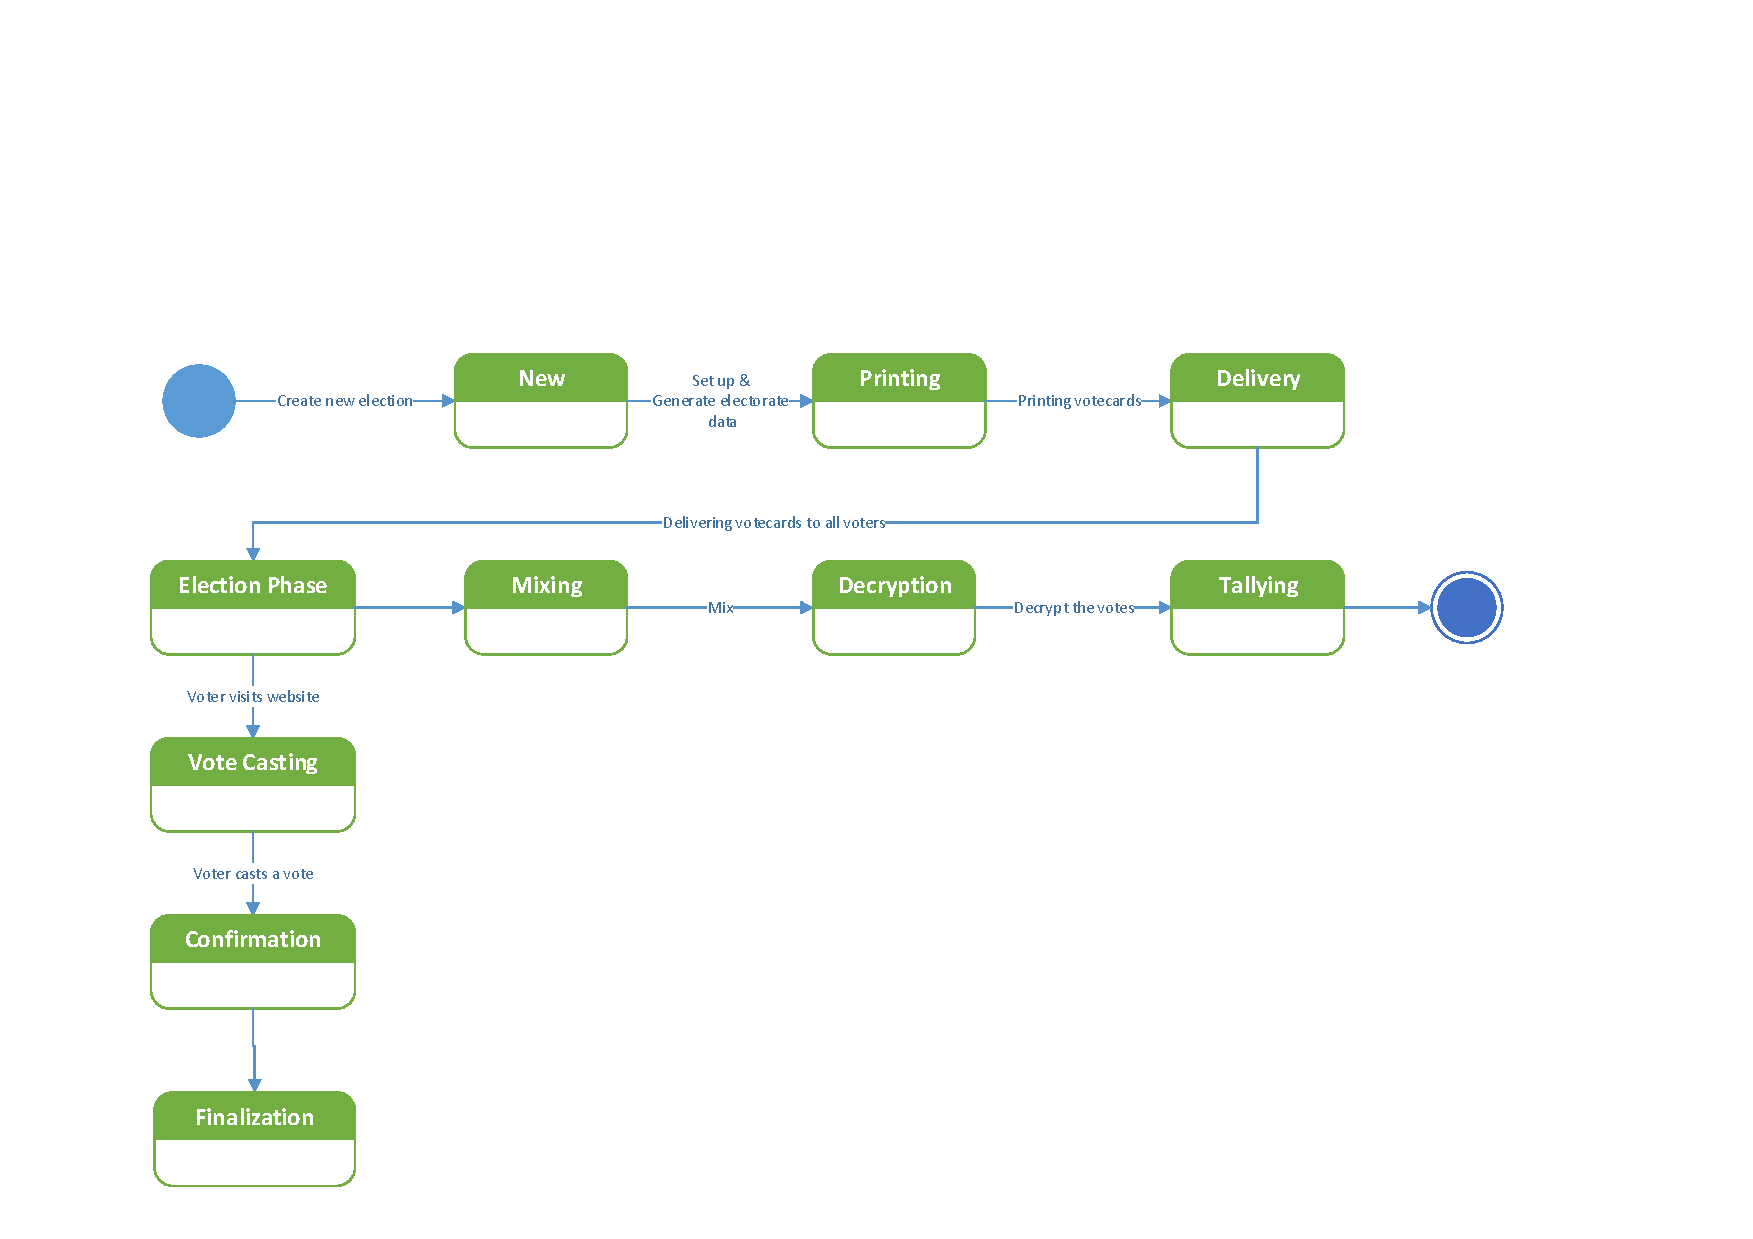
\includegraphics[scale=0.95]{assets/electionStatediagram.pdf}
\caption{System components}
\end{center}
\end{figure}

Each of theses phases consist of one or multiple steps within the CHVote protocol. The election preparation for example, involves the generation of the electorate data based on the input of the election administrator, the public credentials and the public keys. In the specification, these steps are listed as separate actions, however, to reduce the complexity we treat them as one single step in our application. 

As every actor involved in a CHVote election event has it's own set of data to be displayed and specific tasks it has to perform, we decided to create a separate view for every actor, accessible from a tab view displayed on the top of the page.

From the use-cases, we tried to figure out all commonalities between the views:

\begin{itemize}
	\item The views typically display the information known by the respective actor. Especially the bulletin board and election authorities will have a lot of information to be displayed
	\item Almost all views have distinct tasks to be executed by the respective actor, such as casting a ballot in the voters view or confirming ballots from an election authorities view.
  \item The content within each view typically depends on the status an election event is currently in: During the pre-election phase, the vote administrator needs to able to set up the election while in the tallying phase, he must be able to tally and determine the final result.
\end{itemize}
The following matrix shows all the possible combinations:
\begin{figure}[h!]
\begin{center}
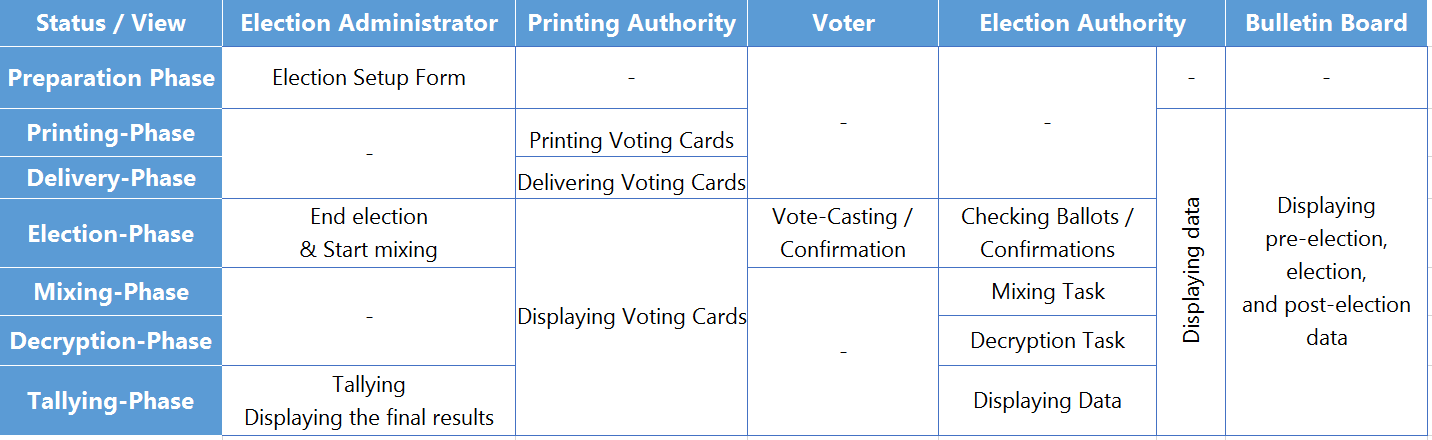
\includegraphics[scale=0.95]{assets/stateactormatrix.png}
\caption{System components}
\end{center}
\end{figure}
Each of the cell values corresponding to one or multiple use-cases.

\section{Design}
Given the rather large amount of complex data to be displayed, the main challenge of the project is a well designed user interface that allows to display all important information while maintaining a clear overview.

To achieve this goal we tried to keep our design very minimalistic and follow the Google material design guidelines as much as possible by choosing an appropriate UI component framework. Even though mobile compatibility hasn't been a requirement, it was nevertheless our goal to make the layout as responsive as possible.

Throughout our application we tried to establish common concepts regarding the look and feel and on how to display our data. One popular layout-concept of the material guidelines is the card layout. Cards can be easily integrated in a responsive grid system, look quite modern and allow to visually group data. In addition, we used pushover menus, tooltips and popups a lot as they made it possible to hide lesser relevant information by default and display it only on demand of the user.

The following screenshots are an extract of the mockups in which we tried to visualize how we imagined the resulting application to look like during the conceptual phase. 

% Todo: Beispiel-Bild der Mockups %

Our conceptual work also involved the development of a small prototype / proof of concept, in which we have implemented one usecase in a reduced extent with the envisaged frameworks to evaluate the technical feasibility. For more information about the languages and frameworks we have decided on, we refer to the next chapter.

\section{Organization}
TODO: Github, Docker, etc.